\documentclass[12pt]{article}  % You can use 10pt, 11pt, or 12pt for font size


\usepackage[utf8]{inputenc}   % Character encoding
\usepackage{amsmath}          % For mathematical typesetting
\usepackage{amsfonts}         % For extra math symbols
\usepackage{amssymb}          % For more math symbols
\usepackage{graphicx}         % To include images
\usepackage{cite}             % For citation management
\usepackage{geometry}         % To adjust page margins
\usepackage{hyperref}         % For clickable links (e.g., references, URLs)
\usepackage{tabularx}

\title{A little more than half a century ago:\\
Mervyn Stone's 1974 paper on cross validation}
\author{Mario Cortina Borja\\
UCL Great Ormond Street Institute of Child Health}  
\date{\today}        % This will display today's date


\begin{document}
\maketitle

 Mervyn Stone (1932--2020) had a distinguished career as Professor of Probability and Statistics, and Head ofthe UCL Department of  Statistical Science; he joined UCL  in 1968.   A list of his publications and an obituary by his friend and colleague at UCL  Rex Galbraith can be seen \href{https://www.ucl.ac.uk/statistics/sites/statistics/files/meryvn-stone-obituary.pdf}{here.}    After retirement, Stone was actively concerned about ``the misuse of statistics in NHS funding formulae and the unwarranted claims made about them'' (Galbraith), and he talks about this in a 2010 interview with him published in \textit{Significance} available \href{https://rss.onlinelibrary.wiley.com/doi/epdf/10.1111/j.1740-9713.2010.00410.x}{here}.   Among his many contributions to UCL,  Galbraith mentions that when the  Department of Statistics, then Department of Statistics and Computer Science, was restructured in 1979 following a split resulting in the Department of Computing Science and the Department of Statistical Science, the latter name was chosen by Stone, then Head of Department.  
 
Many of Stone's publications are remarkable for their deep impact in theoretical and applied statistics, and more recently in science in general, and data science in particular.   
I would like to comment on his pioneer  paper  
\href{https://www.jstor.org/stable/pdf/2984809.pdf?refreqid=fastly-default%3A6cad62e94f9bf73bc0265d3649621bb1&ab_segments=&initiator=&acceptTC=1 }
{ Stone M (1974) Cross--Validatory Choice and Assessment of Statistical Predictions. \textit{JRSS--B}, \textbf{36}: 111--147}  (referred hereafter as S74) which was a discussion paper read in the RSS on December 1973 and published a little more than half a century ago, in January 1974.  There were 13 discussants and their questions and Stone's replies are of very high quality.    

S74 formalises cross--validation (CV) methods;  in particular, the leave-one-out cross validation procedure is firstly defined there.  The paper also deals with generalising estimates of prediction errors. The paper starts with an erudite Introduction providing the historical context in which CV developed.   Stone refers to his preference of the concept of \textit{assessment} of statistical predictions as opposed to \textit{validation}, which ``has a ring of excessive confidence around it'', a semantic distinction which should be borne in mind but seldom is.    Besides the originality of the ideas defined and developed 
the paper has a didactic style.   In section~2
there are numerous theoretical examples further to general statements.   This is followed by a section 
looking at well--known statistical problems, e.g.  predicting the location of a single univariate sample, predictors for the
the $k$--group problem,  and the 
choice of variables for least--squares prediction in which a ``cross-'validatory assessment measure'' is defined.
These examples are defined and analysed in detail through the lens of the methods outlined in the previous section and are then applied to real data.  
The last section discusses the relation of previous work on CV to  the paper's methods, presents a portrait of "a conventional paradigm for a large portion of statistical activity'' including a deviation to consider how the Bayesian paradigm might be accomodated in this scheme, and concudes with a series of quotations addressing philosophical and practical statistical issues.  

There is no substitute to reading the paper to realise its elegance and usefulness but a quick way to demonstrate its growing importance over $50^+$ years is to look at its number of citations and the journals in which papers citing S74 have been published.   I looked at data on such papers obtained from Web of Science (WoS), which claims to be “the world's most trusted publisher-independent global citation database”; 
citations figures were downloaded on 2nd November 2024 and are shown against year of publication 
in Figure~1.  Note that the last point in the Figure does not refer to the definite number of citations for 2024.
Table~1 shows the journals with the largest number of papers citing S74.  There is a clear shift from  S74 being cited in the statistical methods literature to specialised scientific publications, notably in chemometrics, and more recently to being referenced in general science journals.  This process is similar to the three principles of translational medicine: benchside, bedside, and community.  This arc from basic science to generalised scientific practice has been experienced by other important statistical papers, notably by David Cox's 
1972 paper on the \href{https://rss.onlinelibrary.wiley.com/doi/10.1111/j.2517-6161.1972.tb00899.x}
{proportional hazards model} whose remarkable trend in 
number of citations can be
seen  \href{https://rss.onlinelibrary.wiley.com/doi/full/10.1111/1740-9713.01634}{here.}


\begin{figure}[!htp]
\begin{center}
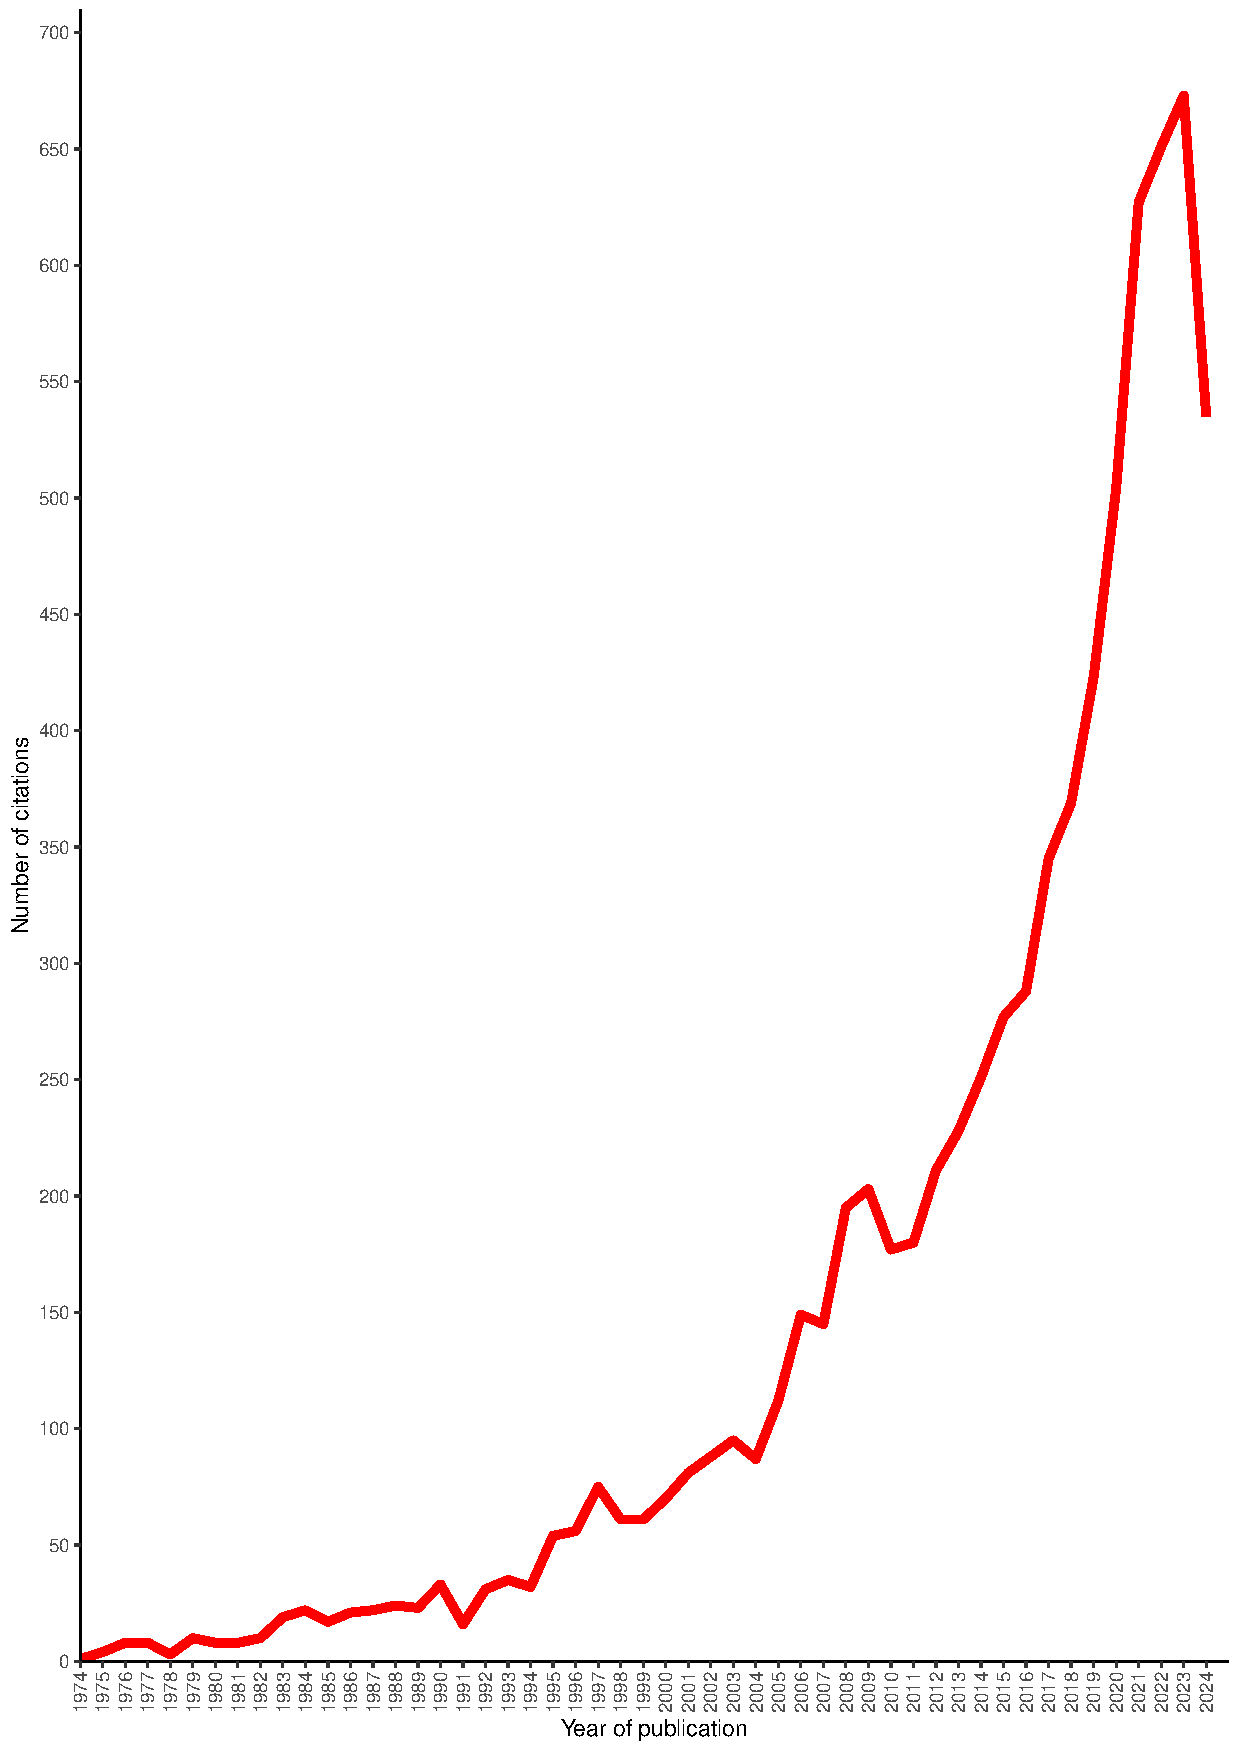
\includegraphics[width = 0.8\textwidth]{S74_Citations.pdf}
\caption{Number of papers citing S74 by year of publication}
\label{figure:S74_Citations}
\end{center}
\end{figure}

\begin{table}[h]
\begin{center}
\begin{tabular}{|lrlr|}
\hline
Year	 &	Number of papers & Publication &		Citations	\\
\hline
1974-1984	&	101 & TECHNOMETRICS	&	10	\\
	&	& J AM STAT ASSOC	&	8	\\
	&	& ANN 	STATS	&	6	\\
	&	& BIOMETRIKA	&	6	\\
	&	& JRSS--B	&	6	\\
	& & JRSS--A	&	4	\\
1985-1994	&254	& J AM STAT ASSOC	&	13	\\
	&	& ANAL CHEM	&	9	\\
	&	& ANN STATS	&	7	\\
	&	& APPL SPECTROSC	&	6	\\
	&	& COMMUN STAT--A	&	6	\\
	&	& J CHEMOMETR	&	6	\\
	&	& JRSS--B	&	6	\\
1995-2004&728 	&	ANAL CHIM ACTA	&	17	\\
   && 	J AM STAT ASSOC	&	14	\\
 	&	& CHEMOMETR INTELL LAB	&	13	\\
	&	& IEEE  T NEURAL NETWOR	&	12	\\
	&	& J CHEMOMETR	&	12	\\
	&	& NEURAL COMPUT	&	12	\\
2005-2014& 1851	&	CHEMOMETR INTELL LAB	&	20	\\
	&& 	PHYS REV--B	&	19	\\
	&& 	NEUROCOMPUTING	&	18	\\
	&& 	EXPERT SYST APPL	&	16	\\
	&	& BMC BIOINFORMATICS	&	13	\\
	&	& COMPUT BIOL MED	&	12	\\
	&& 	PLOS ONE	&	12	\\
2015-2024	& 4692 & 	SUSTAINABILITY	&	83	\\
&	& PLOS ONE	&	50	\\
	&& 	IEEE ACCESS	&	40	\\
	&	& J BUS RES	&	32	\\
	&& 	APPL SCI--BASEL	&	28\\
\hline
\end{tabular}
\caption{Journals with largest number of papers citing S74 by decade of publication}
\end{center}
\end{table}

Mervyn Stone played an important role in UCL, and his contributions to the theory and application of statistical methods continue to be increasingly useful in many scientific areas.  
I hope this short paper draws attention to his life and work.

\end{document}


